\documentclass{beamer}
\mode<presentation>
{
	\usetheme{Madrid}
    
    \definecolor{unisinos}{RGB}{67,40,117}
    \usecolortheme[named=unisinos]{structure}
    
	\usefonttheme{professionalfonts}
    \usebackgroundtemplate{
\includegraphics[width=\paperwidth,height=0.978\paperheight]{template_unisinos}}

 	\beamertemplatenavigationsymbolsempty
 	\setbeamertemplate{footline}
	{
	  \leavevmode%
	  \hbox{%
	  \begin{beamercolorbox}[wd=.12\paperwidth,ht=2.25ex,dp=1ex,center]{author in head/foot}%
	    \usebeamerfont{author in head/foot}\insertshortauthor
	  \end{beamercolorbox}%
	  \begin{beamercolorbox}[wd=.88\paperwidth,ht=2.25ex,dp=1ex,center]{title in head/foot}%
	    \usebeamerfont{title in head/foot}\insertshorttitle\hspace*{3em}
	    \insertframenumber{} / \inserttotalframenumber\hspace*{1ex}
	  \end{beamercolorbox}}%
	  \vskip0pt%
	}
 	\setbeamertemplate{caption}[numbered]
 	\usepackage{caption}

 	\usepackage[brazil]{babel}		% Idioma do documento
	\usepackage{siunitx}
	\usepackage{ragged2e}
	\usepackage{float}
    \usepackage{indentfirst} }
    \usepackage[alf]{abntex2cite}		% Citações padrão ABNT
	\usepackage{color}			% Controle das cores
	\usepackage[T1]{fontenc}		% Selecao de codigos de fonte.
	\usepackage{graphicx}			% Inclusão de gráficos
	\usepackage[utf8]{inputenc}		% Codificacao do documento (conversão automática dos acentos)
	\usepackage{txfonts}			% Fontes virtuais

	\usepackage{movie15}

\title[ Desenvolvimento de um Controlador PID com Auto Sintonia usando Redes Neurais Artificiais e Regressão ...]{Desenvolvimento de um Controlador PID com Auto Sintonia usando Redes Neurais Artificiais e Regressão Não-Linear Robusta para o Controle de Atitude de um Simulador de Satélites com
Rodas de Reação}
\author[Piaia, G. A.]{
	{\fontsize{10}{8}\selectfont \textbf{Aluno:} Guilherme Angelo Piaia} \\
	{\fontsize{10}{8}\selectfont \textbf{Orientador}: Rodrigo Marques de Figueiredo}
}
%\institute[UNISINOS]{UNISINOS - Universidade do Vale do Rio dos Sinos \\ Engenharia de Controle e Automação}

\date{\today}

\begin{document}

%%%%%%%%%%%%%%%%%%%%%%%%%%%%%%%%%%%

\begin{frame}
	\begin{minipage}{1\linewidth}
		\centering
		    \textbf{UNISINOS - Universidade do Vale do Rio dos Sinos} \\ Engenharia de Controle e Automação
	\end{minipage}
	\titlepage
\end{frame}

%%%%%%%%%%%%%%%%%%%%%%%%%%%%%%%%%%%

\begin{frame}{Sumário}
	\tableofcontents
\end{frame}

%%%%%%%%%%%%%%%%%%%%%%%%%%%%%%%%%%%

\begin{frame}{Introdução}
    \begin{figure}[HT]
		\begin{center}
		\captionsetup{justification=centering}
        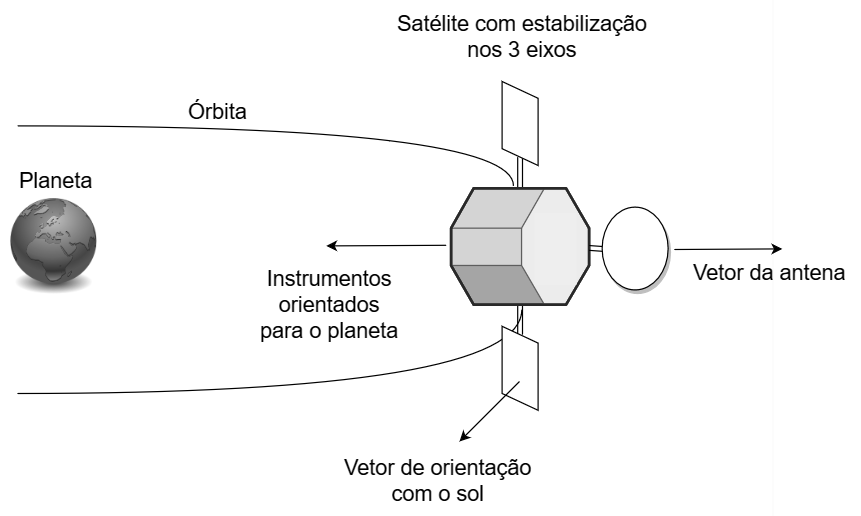
\includegraphics[scale=.42]{../referencial/img/rotational_brown_p256}
        \caption{Movimento de translação de um satélite artificial. \newline
        		 Fonte: Adaptado de \citeonline{Brown2002}.}
		\label{FIG_ADAPTATIVO}
        \end{center}
	\end{figure}
\end{frame}

%%%%%%%%%%%%%%%%%%%%%%%%%%%%%%%%%%%

\section{Introdução}
\begin{frame}{Introdução}
	\begin{itemize}
		\justifying
		\item O controle acurado da posição é
necessário para manter o alinhamento com o planeta ou alvo. 
		\item Uma das formas de se controlar a posição de um satélite é através da variação do momento angular de rodas.
		\item Diversas técnicas de controle são empregadas para se controlar essa posição. O tipo mais usado é o controlador PID  (Proporcional-Integral-Derivativo).
		\item Esses controladores necessitam de sintonia para que tenham uma performance satisfatória.
		\item Este trabalho tem por principal objetivo a implementação em um sistema embarcado
de um controlador com sintonia automática utilizando conceitos de controle inteligente e testa-lo em um simulador de satélites com rodas de reação.
    \end{itemize}
\end{frame}

%%%%%%%%%%%%%%%%%%%%%%%%%%%%%%%%%%%
\section{Referencial Teórico}
\begin{frame}{Referencial Teórico - Mecânica de corpo rígido}
	\begin{itemize}
		\justifying
		\item Para a modelagem, partimos do princípio do torque ($\vec{\tau}$) gerado pela variação instantânea do momento angular ($\dot{\vec{L}}$):
    \end{itemize}

	\begin{itemize}
		\justifying
		\item Onde o momento angular pode ser descrito da seguinte forma:
    \end{itemize}

	\begin{equation}\label{eq:iomega}
		\vec{L}=I\vec{\omega}
	\end{equation}

	\begin{itemize}
		\justifying
		\item Sendo $I$ o momento de inércia e $\vec{\omega}$ o vetor velocidade angular.
    \end{itemize}


\end{frame}

%%%%%%%%%%%%%%%%%%%%%%%%%%%%%%%%%%%

\begin{frame}{Referencial Teórico - Mecânica de corpo rígido}
	\begin{itemize}
		\justifying
		\item Após a devida modelagem, conseguimos relacionar os torques ($\tau_{1}$, $\tau_{2}$ e $\tau_{3}$), momentos de inércia em cada eixo (A, B e C) com as derivadas primeiras das velocidades angulares ($\dot{\omega_{1}}$, $\dot{\omega_{2}}$ e $\dot{\omega_{3}}$) 
    \end{itemize}

	\begin{equation}
	  \dot{\omega_{1}}=\frac{\tau_{1}}{A}+\left(\frac{B-C}{A}\right)\omega_{2}\omega_{3}
	\end{equation}
	\begin{equation}
	  \dot{\omega_{2}}=\frac{\tau_{2}}{B}+\left(\frac{C-A}{B}\right)\omega_{1}\omega_{3}
	\end{equation}
	\begin{equation}
	  \dot{\omega_{3}}=\frac{\tau_{2}}{C}+\left(\frac{A-B}{C}\right)\omega_{1}\omega_{2}
	\end{equation}
\end{frame}

%%%%%%%%%%%%%%%%%%%%%%%%%%%%%%%%%%%

\begin{frame}{Referencial Teórico - Rodas de Reação}
    \begin{figure}[HT]
		\begin{center}
		\captionsetup{justification=centering}
        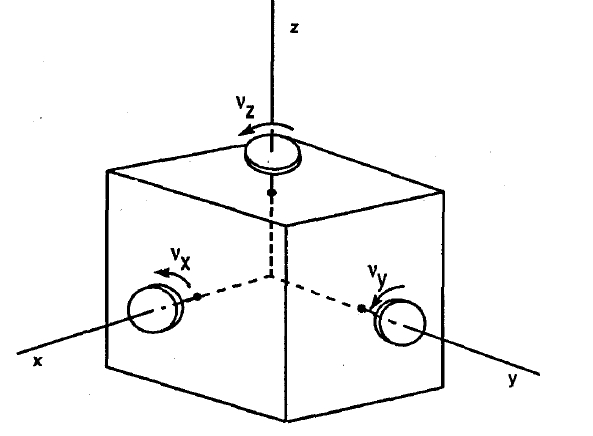
\includegraphics[scale=.42]{../referencial/img/satellite_controlhand_p1306}
        \caption{Representação de um corpo rígido com rodas de reação. \newline
        		 Fonte: Adaptado de \citeonline{Levine1996}.}
		\label{FIG_ADAPTATIVO}
        \end{center}
	\end{figure}
\end{frame}

%%%%%%%%%%%%%%%%%%%%%%%%%%%%%%%%%%%

\begin{frame}{Referencial Teórico - Rodas de Reação}
	\begin{itemize}
		\justifying
		\item Princípio da conservação do momento angular:
    \end{itemize}

	\begin{equation}\label{eq:ltot}
		\vec{L}_{total}=\vec{L}_s+\vec{L}_{\omega}=constante 
	\end{equation}

		\begin{itemize}
		\justifying
		\item E se substituirmos o torque pela seguinte relação:
    \end{itemize}
       \begin{equation}
		\vec{\tau}=\dot{\vec{L}}
	\end{equation}

	\begin{itemize}
		\justifying
		\item No próximo slide temos a relação mais apropriada para a modelagem.
    \end{itemize}
\end{frame}

%%%%%%%%%%%%%%%%%%%%%%%%%%%%%%%%%%%

\begin{frame}{Referencial Teórico - Rodas de Reação}

	\begin{equation}\label{eq:modeloA}
	  \dot{\omega_{1}}=\frac{J_{\omega 1}\dot{\vec{\psi}}_{\omega 1}}{A}+\left(\frac{B-C}{A}\right)\omega_{2}\omega_{3}
	\end{equation}

	\begin{equation}\label{eq:modeloB}
	  \dot{\omega_{2}}=\frac{J_{\omega 2}\dot{\vec{\psi}}_{\omega 2}}{B}+\left(\frac{C-A}{B}\right)\omega_{1}\omega_{3}
	\end{equation}

	\begin{equation}\label{eq:modeloC}
	  \dot{\omega_{3}}=\frac{J_{\omega 3}\dot{\vec{\psi}}_{\omega 3}}{C}+\left(\frac{A-B}{C}\right)\omega_{1}\omega_{2}
	\end{equation}

	\begin{itemize}
		\justifying
		\item Assim, conseguimos relacionar o momento angular das rodas ($J_{\omega 1}$, $J_{\omega 2}$ e $J_{\omega 3}$) com a derivada da velocidade das mesmas ($\dot{\vec{\psi}}_{\omega 1}$, $\dot{\vec{\psi}}_{\omega 2}$ e $\dot{\vec{\psi}}_{\omega 3}$).
    \end{itemize}

\end{frame}

%%%%%%%%%%%%%%%%%%%%%%%%%%%%%%%%%%%

\begin{frame}{Referencial Teórico - Controle}
    \begin{figure}[HT]
		\begin{center}
		\captionsetup{justification=centering}
        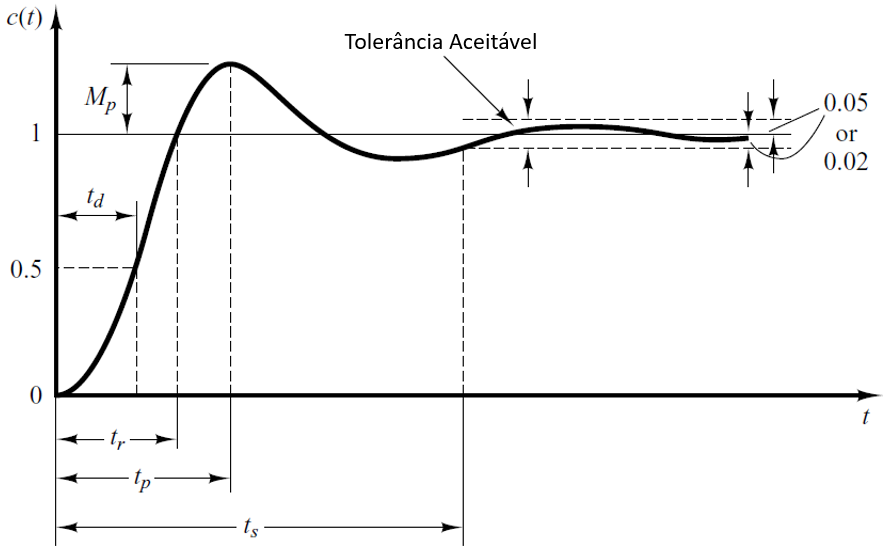
\includegraphics[scale=.35]{../referencial/img/transient_ogata_p170}
        \caption{Parâmetros de uma resposta ao degrau de um sistema de segunda ordem ou superior. \newline
        		 Fonte: Adaptado de \citeonline{Ogata}.}
		\label{FIG_ADAPTATIVO}
        \end{center}
	\end{figure}
\end{frame}

%%%%%%%%%%%%%%%%%%%%%%%%%%%%%%%%%%%

\begin{frame}{Referencial Teórico - Controle}
    \begin{figure}[HT]
		\begin{center}
		\captionsetup{justification=centering}
        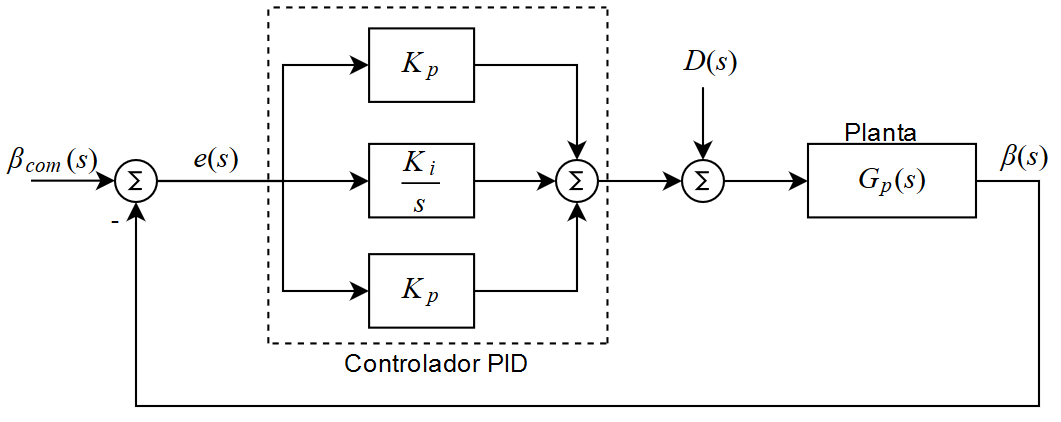
\includegraphics[scale=.45]{../referencial/img/pid_controller_Snider_p35}
        \caption{Representação do modelo paralelo de um controlador PID com distúrbios. \newline
        		 Fonte: Elaborado pelo autor}
		\label{FIG_ADAPTATIVO}
        \end{center}
	\end{figure}
\end{frame}

%%%%%%%%%%%%%%%%%%%%%%%%%%%%%%%%%%%

\begin{frame}{Referencial Teórico - Método Clássico de Sintonia}
    \begin{figure}[HT]
		\begin{center}
		\captionsetup{justification=centering}
        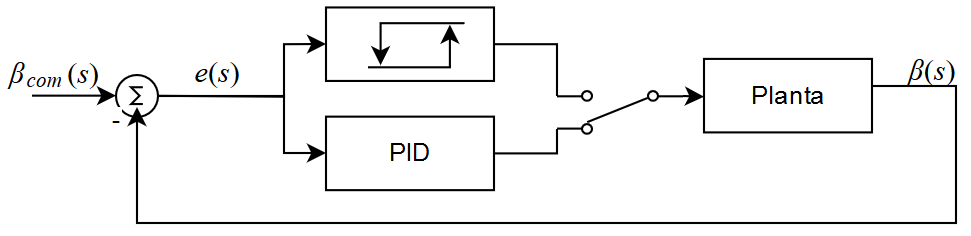
\includegraphics[scale=.3]{../referencial/img/pid_autotuning_relay_astrom_p239}
        \caption{Modelo do método de auto sintonia via relé. \newline
        		 Fonte: Adaptado de \citeonline{Astrom1995}.}
		\label{FIG_ADAPTATIVO}
        \end{center}
	\end{figure}
\begin{columns}
    \begin{column}{0.50\textwidth}
	\begin{itemize}
		\item O ganho crítico $K_u$ pode ser encontrado da seguinte forma:
	\end{itemize}
	\begin{equation}\label{eq:n(a)}
	  K_u=\frac{4d}{\pi a}\left(\sqrt{1-\left(\frac{\varepsilon}{a}\right)^{2}}-i\frac{\varepsilon}{a}\right) 
	\end{equation}
    \end{column}
    \begin{column}{0.5\textwidth}

	\begin{itemize}
	\item Onde \textit{d} é a amplitude de oscilação do relé, \textit{$\varepsilon$} é a histerese do relé e \textit{$a$} é a amplitude de oscilação da saída \cite{Levine1996}.
	\end{itemize}
	\end{column}
\end{columns}
\end{frame}

%%%%%%%%%%%%%%%%%%%%%%%%%%%%%%%%%%%

\begin{frame}{Referencial Teórico - Estado da Arte}
    \begin{figure}[HT]
		\begin{center}
		\captionsetup{justification=centering}
        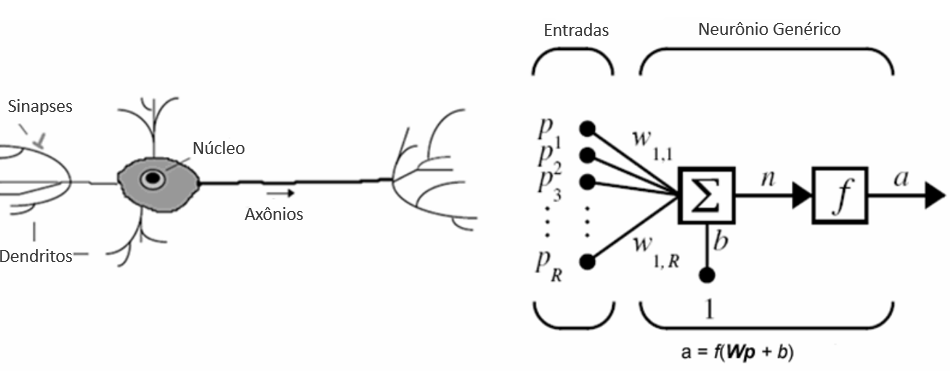
\includegraphics[scale=.35]{../referencial/img/neuronio_unal_p6}
        \caption{Célula de um neurônio natural e modelo matemático respectivo. \newline
        		 Fonte: Adaptado de  \citeonline{Unal2013}.}
		\label{FIG_ADAPTATIVO}
        \end{center}
	\end{figure}
\end{frame}

%%%%%%%%%%%%%%%%%%%%%%%%%%%%%%%%%%%

\begin{frame}{Referencial Teórico - Estado da Arte}
    \begin{figure}[HT]
		\begin{center}
		\captionsetup{justification=centering}
        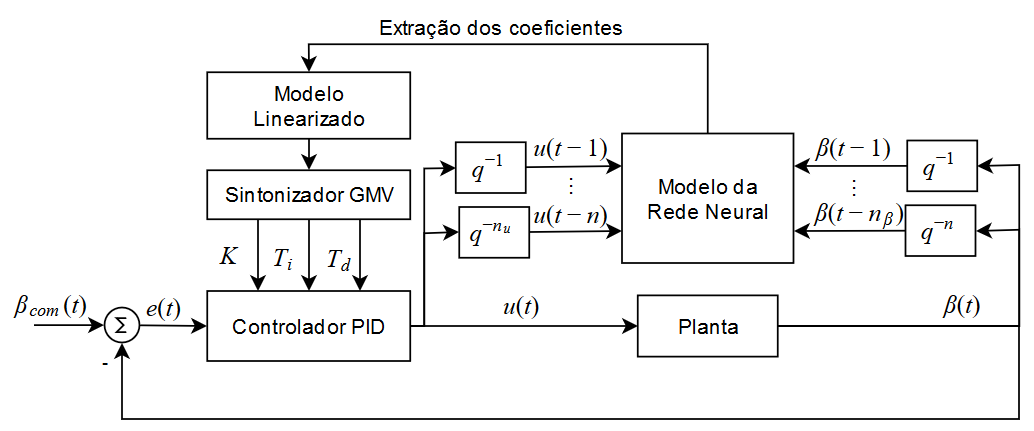
\includegraphics[scale=.42]{../referencial/img/pid_neural_chen_p212}
        \caption{Controlador PID com rede neural. \newline
        		 Fonte: Adaptado de \citeonline{Chen2004}.}
		\label{FIG_ADAPTATIVO}
        \end{center}
	\end{figure}
\end{frame}

%%%%%%%%%%%%%%%%%%%%%%%%%%%%%%%%%%%
\section{Metodologia}
\begin{frame}{Metodologia - Hardware}

\begin{columns}
    \begin{column}{0.50\textwidth}
    \begin{figure}[HT]
		\begin{center}
		\captionsetup{justification=centering}
        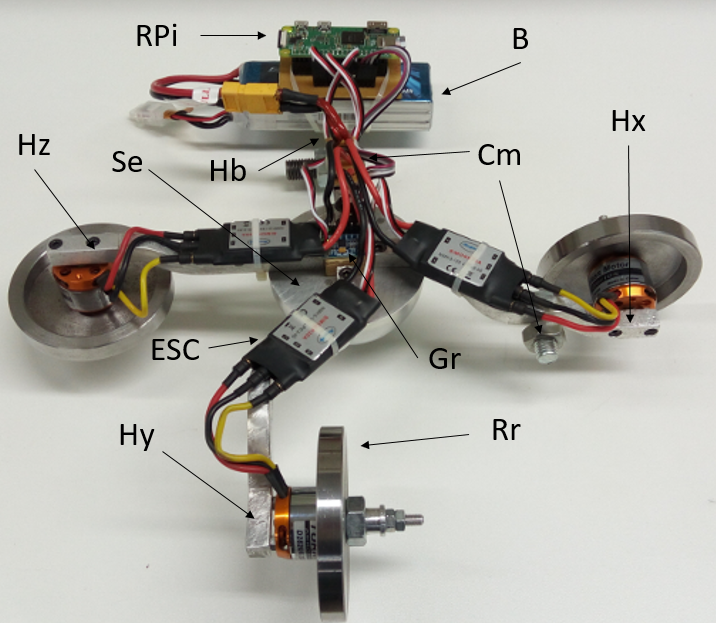
\includegraphics[scale=.3]{../metodologia/img/corpo_real}
        \caption{Corpo do simulador de satélites prototipado. \newline
        		 Fonte: Elaborado pelo autor.}
		\label{FIG_ADAPTATIVO}
        \end{center}
	\end{figure}
    \end{column}
    \begin{column}{0.5\textwidth}

	\begin{itemize}
    	\justifying
    	\item Hx, Hy e Hz são as hastes nos 3 eixos cartesianos
    	\item Hb é a haste da bateria
    	\item ESC são os drivers para os motores sem escovas
    	\item Rr são as rodas de reação
    	\item Se é a esfera que compõe o mancal
    	\item RPi é a Raspberry Pi Zero W
    	\item Cm são as compensações de massa
    	\item Gr é o giroscópio e B é a bateria
    \end{itemize}
    \end{column}
\end{columns}
\end{frame}

%%%%%%%%%%%%%%%%%%%%%%%%%%%%%%%%%%%

\begin{frame}{Metodologia - Hardware}
	\begin{itemize}
		\justifying
    	\item \href{https://youtu.be/TpdmkFmt9iw}{\beamergotobutton{Vídeo do primeiro teste do mancal}}
    \end{itemize}
    \begin{figure}[HT]
		\begin{center}
		\captionsetup{justification=centering}
        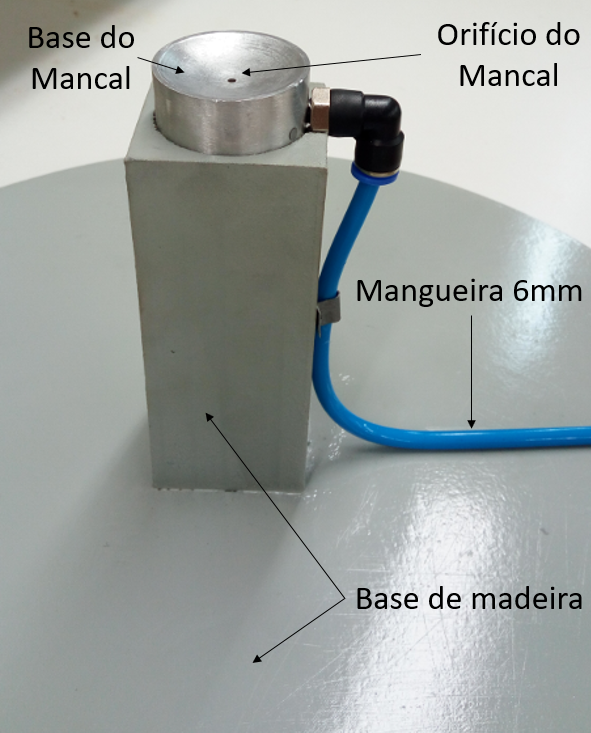
\includegraphics[scale=.25]{../metodologia/img/base_real}
        \caption{Base do simulador de satélites prototipado. \newline
        		 Fonte: Elaborado pelo autor.}
		\label{FIG_ADAPTATIVO}
        \end{center}
	\end{figure}	

\end{frame}

%%%%%%%%%%%%%%%%%%%%%%%%%%%%%%%%%%%

\begin{frame}{Metodologia - Hardware}
    \begin{figure}[HT]
		\begin{center}
		\captionsetup{justification=centering}
        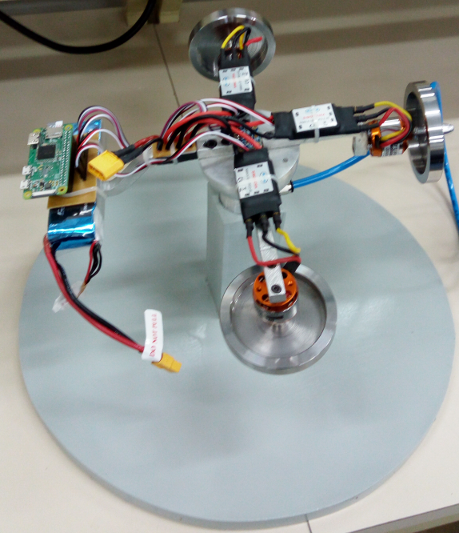
\includegraphics[scale=.3]{../metodologia/img/simulador_real}
        \caption{Simulador de satélites prototipado. \newline
        		 Fonte: Elaborado pelo autor.}
		\label{FIG_ADAPTATIVO}
        \end{center}
	\end{figure}
\end{frame}

%%%%%%%%%%%%%%%%%%%%%%%%%%%%%%%%%%%

\begin{frame}{Metodologia - Modelo do Motor-Roda}

\begin{columns}
    \begin{column}{0.40\textwidth}
        \begin{figure}[HT]
		\begin{center}
		\captionsetup{justification=centering}
        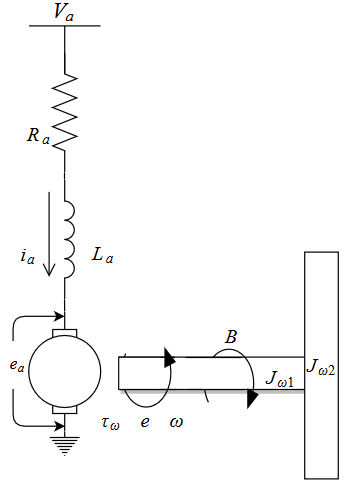
\includegraphics[scale=.4]{../metodologia/img/modelo_motor_dc}
        \caption{Modelo do motor DC. \newline
        		 Fonte: Elaborado pelo autor.}
		\label{FIG_ADAPTATIVO}
        \end{center}
	\end{figure}
    \end{column}
    \begin{column}{0.60\textwidth}

	\begin{equation}\label{eq:motor_accel}
	  	\frac{\dot{\omega}(s)}{V_a(s)} = \frac{K_wK_t s}{(R_a+ Las)(Js+B)+K_wK_t}  
	\end{equation}
	\begin{itemize}
    	\justifying
    	\item Onde $R_a$, $L_a$, $i_a$ e $e_a$ são a resistência, a indutância, a corrente e a tensão de armadura, respectivamente, $e_b$ é a tensão induzida. $\tau_{\omega}$ é o torque do motor, $\dot{\omega}$ é a derivada da velocidade angular, $K_t$ é a constante de torque, $K_w$ é a constante de velocidade contra-eletromotriz, J é i momento de inércia motor-roda, $V_a$ é tensão da fonte e B é o atrito viscoso.
    \end{itemize}
    \end{column}
\end{columns}
\end{frame}

%%%%%%%%%%%%%%%%%%%%%%%%%%%%%%%%%%%

\begin{frame}{Metodologia - Sistema de controle}
    \begin{figure}[HT]
		\begin{center}
		\captionsetup{justification=centering}
        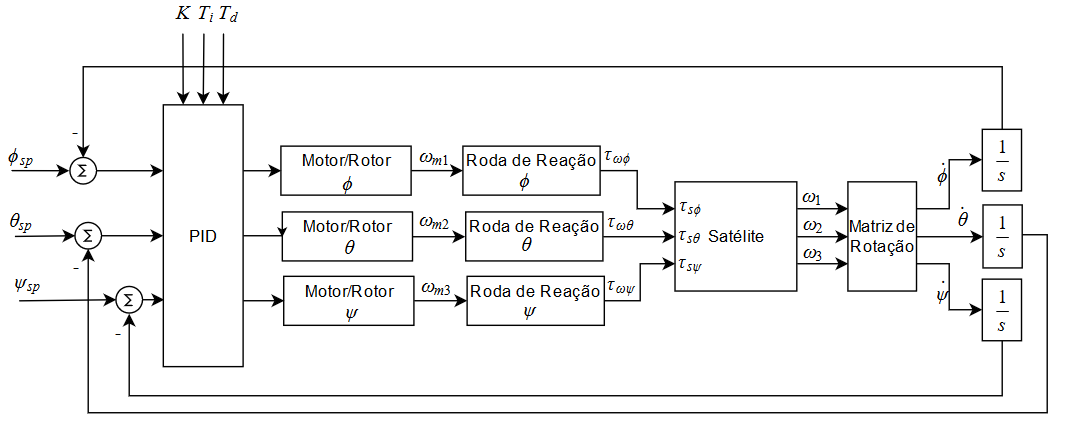
\includegraphics[scale=.42]{../metodologia/img/modelo_satelite_pid}
        \caption{Modelo em malha fechada com um controlador PID. \newline
        		 Fonte: Elaborado pelo autor.}
		\label{FIG_ADAPTATIVO}
        \end{center}
	\end{figure}
\end{frame}

%%%%%%%%%%%%%%%%%%%%%%%%%%%%%%%%%%%

\begin{frame}{Metodologia - Sistema de controle}
    \begin{figure}[HT]
		\begin{center}
		\captionsetup{justification=centering}
        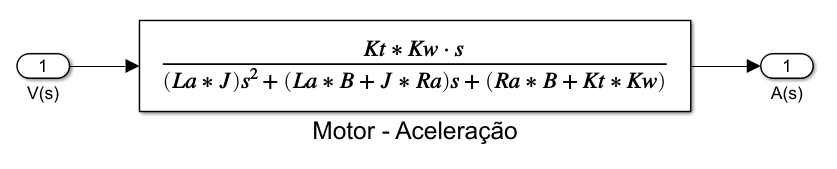
\includegraphics[scale=.25]{../metodologia/img/modelo_satelite_motor}
        \caption{Função de transferência dos motores. \newline
        		 Fonte: Elaborado pelo autor.}
		\label{FIG_ADAPTATIVO}
        \end{center}
	\end{figure}

    \begin{figure}[HT]
		\begin{center}
		\captionsetup{justification=centering}
        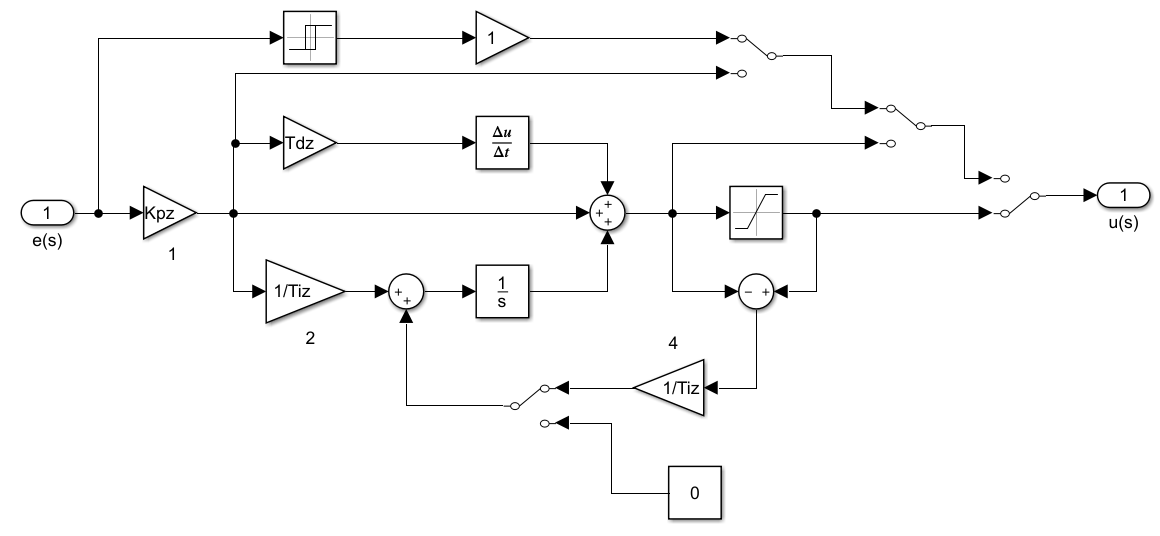
\includegraphics[scale=.25]{../metodologia/img/matlab_pid_antiwindup}
        \caption{Digrama de blocos do controlador PID com Anti-Windup. \newline
        		 Fonte: Elaborado pelo autor.}
		\label{FIG_ADAPTATIVO}
        \end{center}
	\end{figure}
\end{frame}

%%%%%%%%%%%%%%%%%%%%%%%%%%%%%%%%%%%

\begin{frame}{Metodologia - Software}
    \begin{figure}[HT]
		\begin{center}
		\captionsetup{justification=centering}
        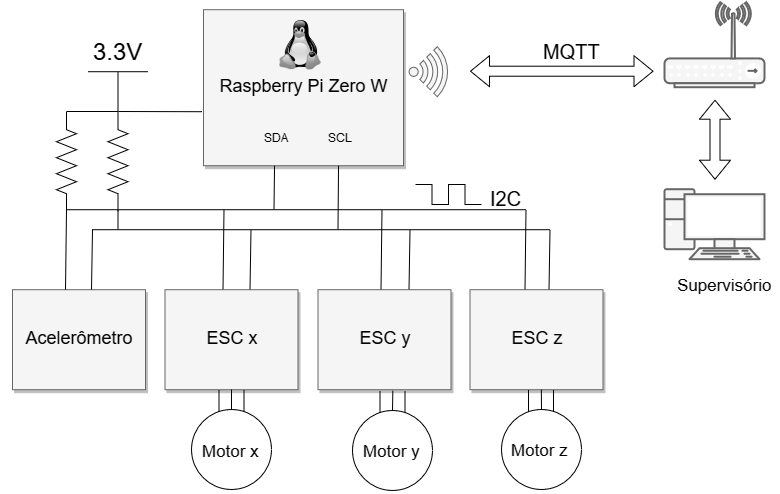
\includegraphics[scale=.45]{../metodologia/img/comunicacao_projeto}
        \caption{Representação geral do sistema. \newline
        		 Fonte: Elaborado pelo autor.}
		\label{FIG_ADAPTATIVO}
        \end{center}
	\end{figure}
\end{frame}

%%%%%%%%%%%%%%%%%%%%%%%%%%%%%%%%%%%

\begin{frame}{Metodologia - Software}
    \begin{figure}[HT]
		\begin{center}
		\captionsetup{justification=centering}
        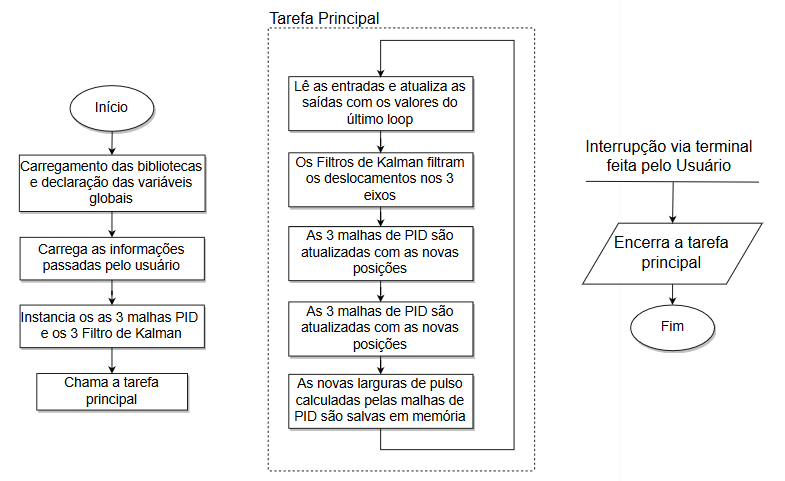
\includegraphics[scale=.45]{../metodologia/img/software_model}
        \caption{Fluxograma do software de controle. \newline
        		 Fonte: Elaborado pelo autor.}
		\label{fig:software_model}
        \end{center}
	\end{figure}
\end{frame}

%%%%%%%%%%%%%%%%%%%%%%%%%%%%%%%%%%%

\begin{frame}{Metodologia - Software}
    \begin{figure}[HT]
		\begin{center}
		\captionsetup{justification=centering}
        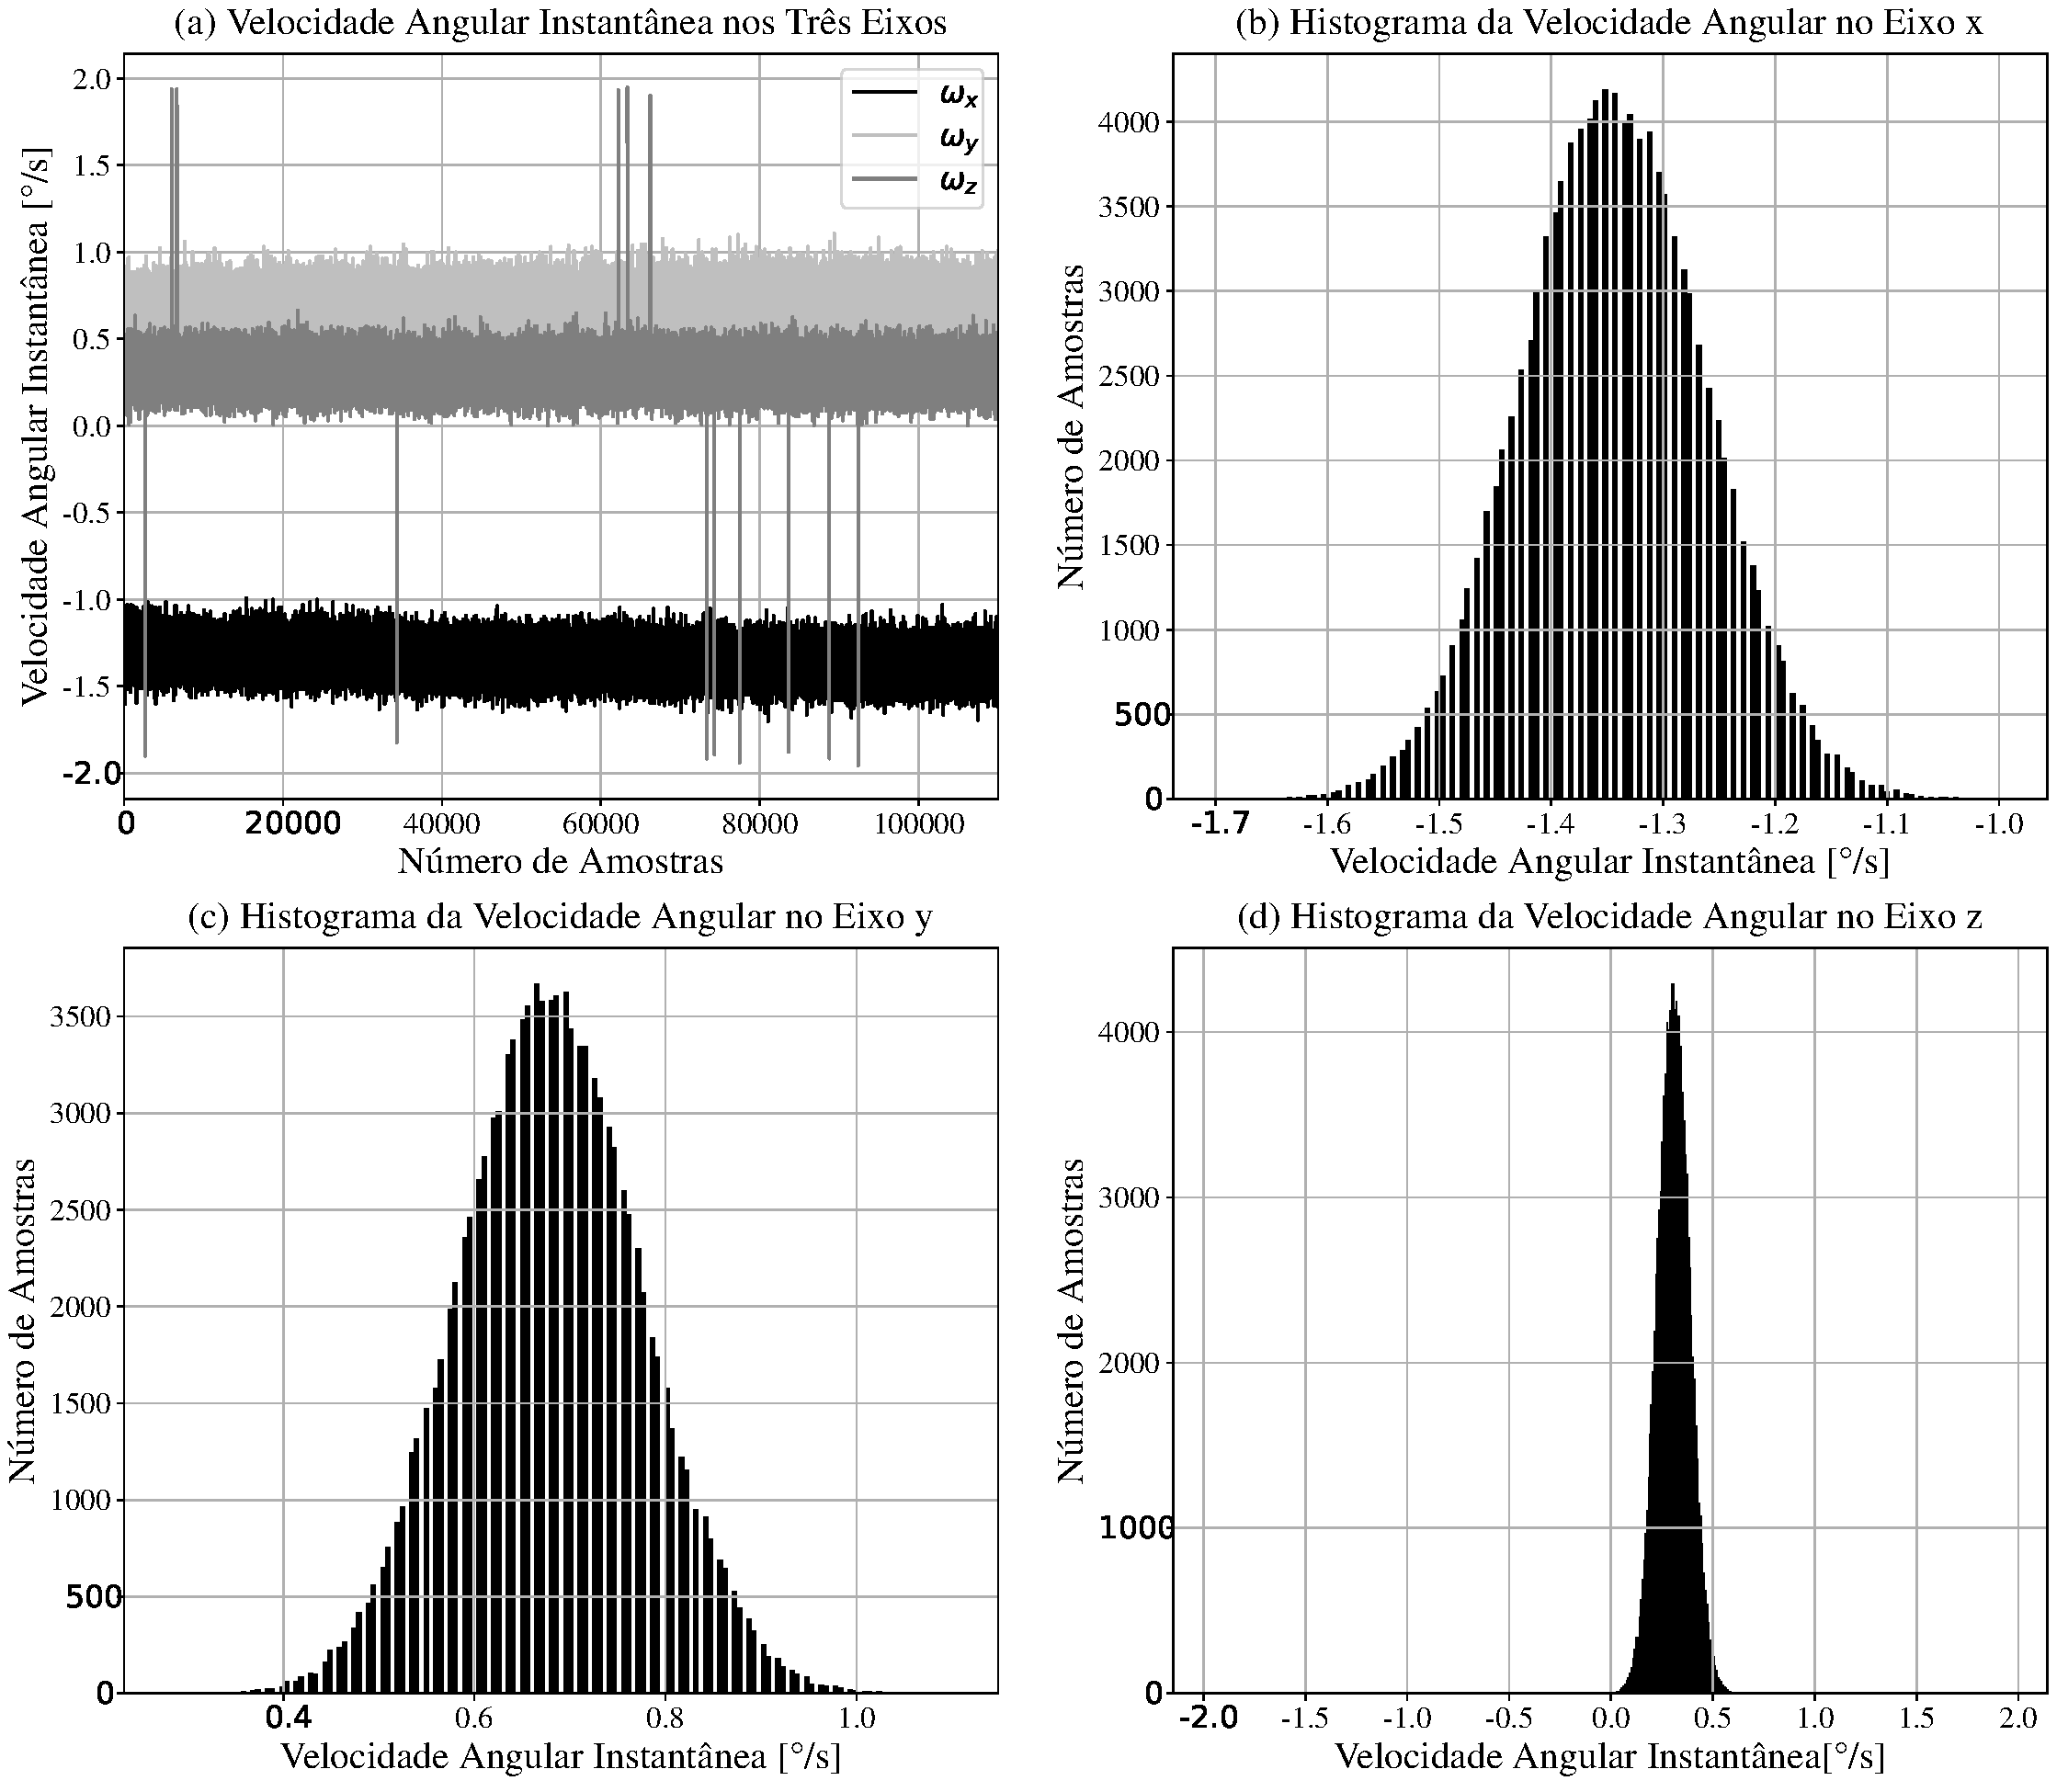
\includegraphics[scale=.17]{../metodologia/img/bias_correction}
        \caption{Características dos sinais amostrados pelo giroscópio. \newline
        		 Fonte: Elaborado pelo autor.}
		\label{FIG_ADAPTATIVO}
        \end{center}
	\end{figure}
\end{frame}

%%%%%%%%%%%%%%%%%%%%%%%%%%%%%%%%%%%

\begin{frame}{Metodologia - RNA e Regressão Não-Linear}
    \begin{figure}[HT]
		\begin{center}
		\captionsetup{justification=centering}
        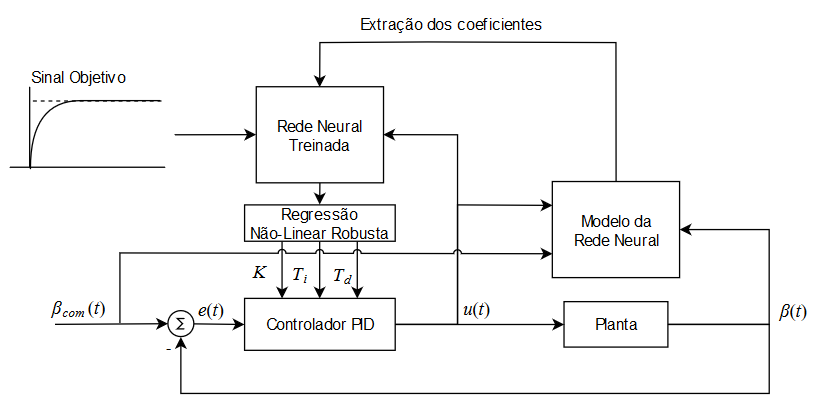
\includegraphics[scale=.5]{../metodologia/img/neural_regression}
        \caption{Diagrama de blocos do sintonizador e otimizador. \newline
        		 Fonte: Elaborado pelo autor.}
		\label{fig:neural_regression}
        \end{center}
	\end{figure}
\end{frame}

%%%%%%%%%%%%%%%%%%%%%%%%%%%%%%%%%%%

\section{Análise dos Resultados}
\begin{frame}{Análise dos Resultados}
	\begin{itemize}
		\justifying
		\item Passos executados durante os testes:
		\begin{itemize}
			\item Treinamento da RNA com um ganho proporcional unitário e posterior otimização dos parâmetros para uma operação inicial.
			\item Método clássico de sintonia usando o método do relé.
			\item Execução de ensaios com todos os parâmetros calculados.
		\end{itemize}

		\item \href{https://youtu.be/cbJlq2HjHKE}{\beamergotobutton{Vídeo do sistema marginalmente estável}} \newline
		\item \href{https://youtu.be/Aj6VIQYChpI}{\beamergotobutton{Vídeo da resposta ao degrau}}
	\end{itemize}
\end{frame}

%%%%%%%%%%%%%%%%%%%%%%%%%%%%%%%%%%%

\begin{frame}{Análise dos Resultados - Treinamento da RNA}
     \begin{figure}[HT]
		\begin{center}
		\captionsetup{justification=centering}
        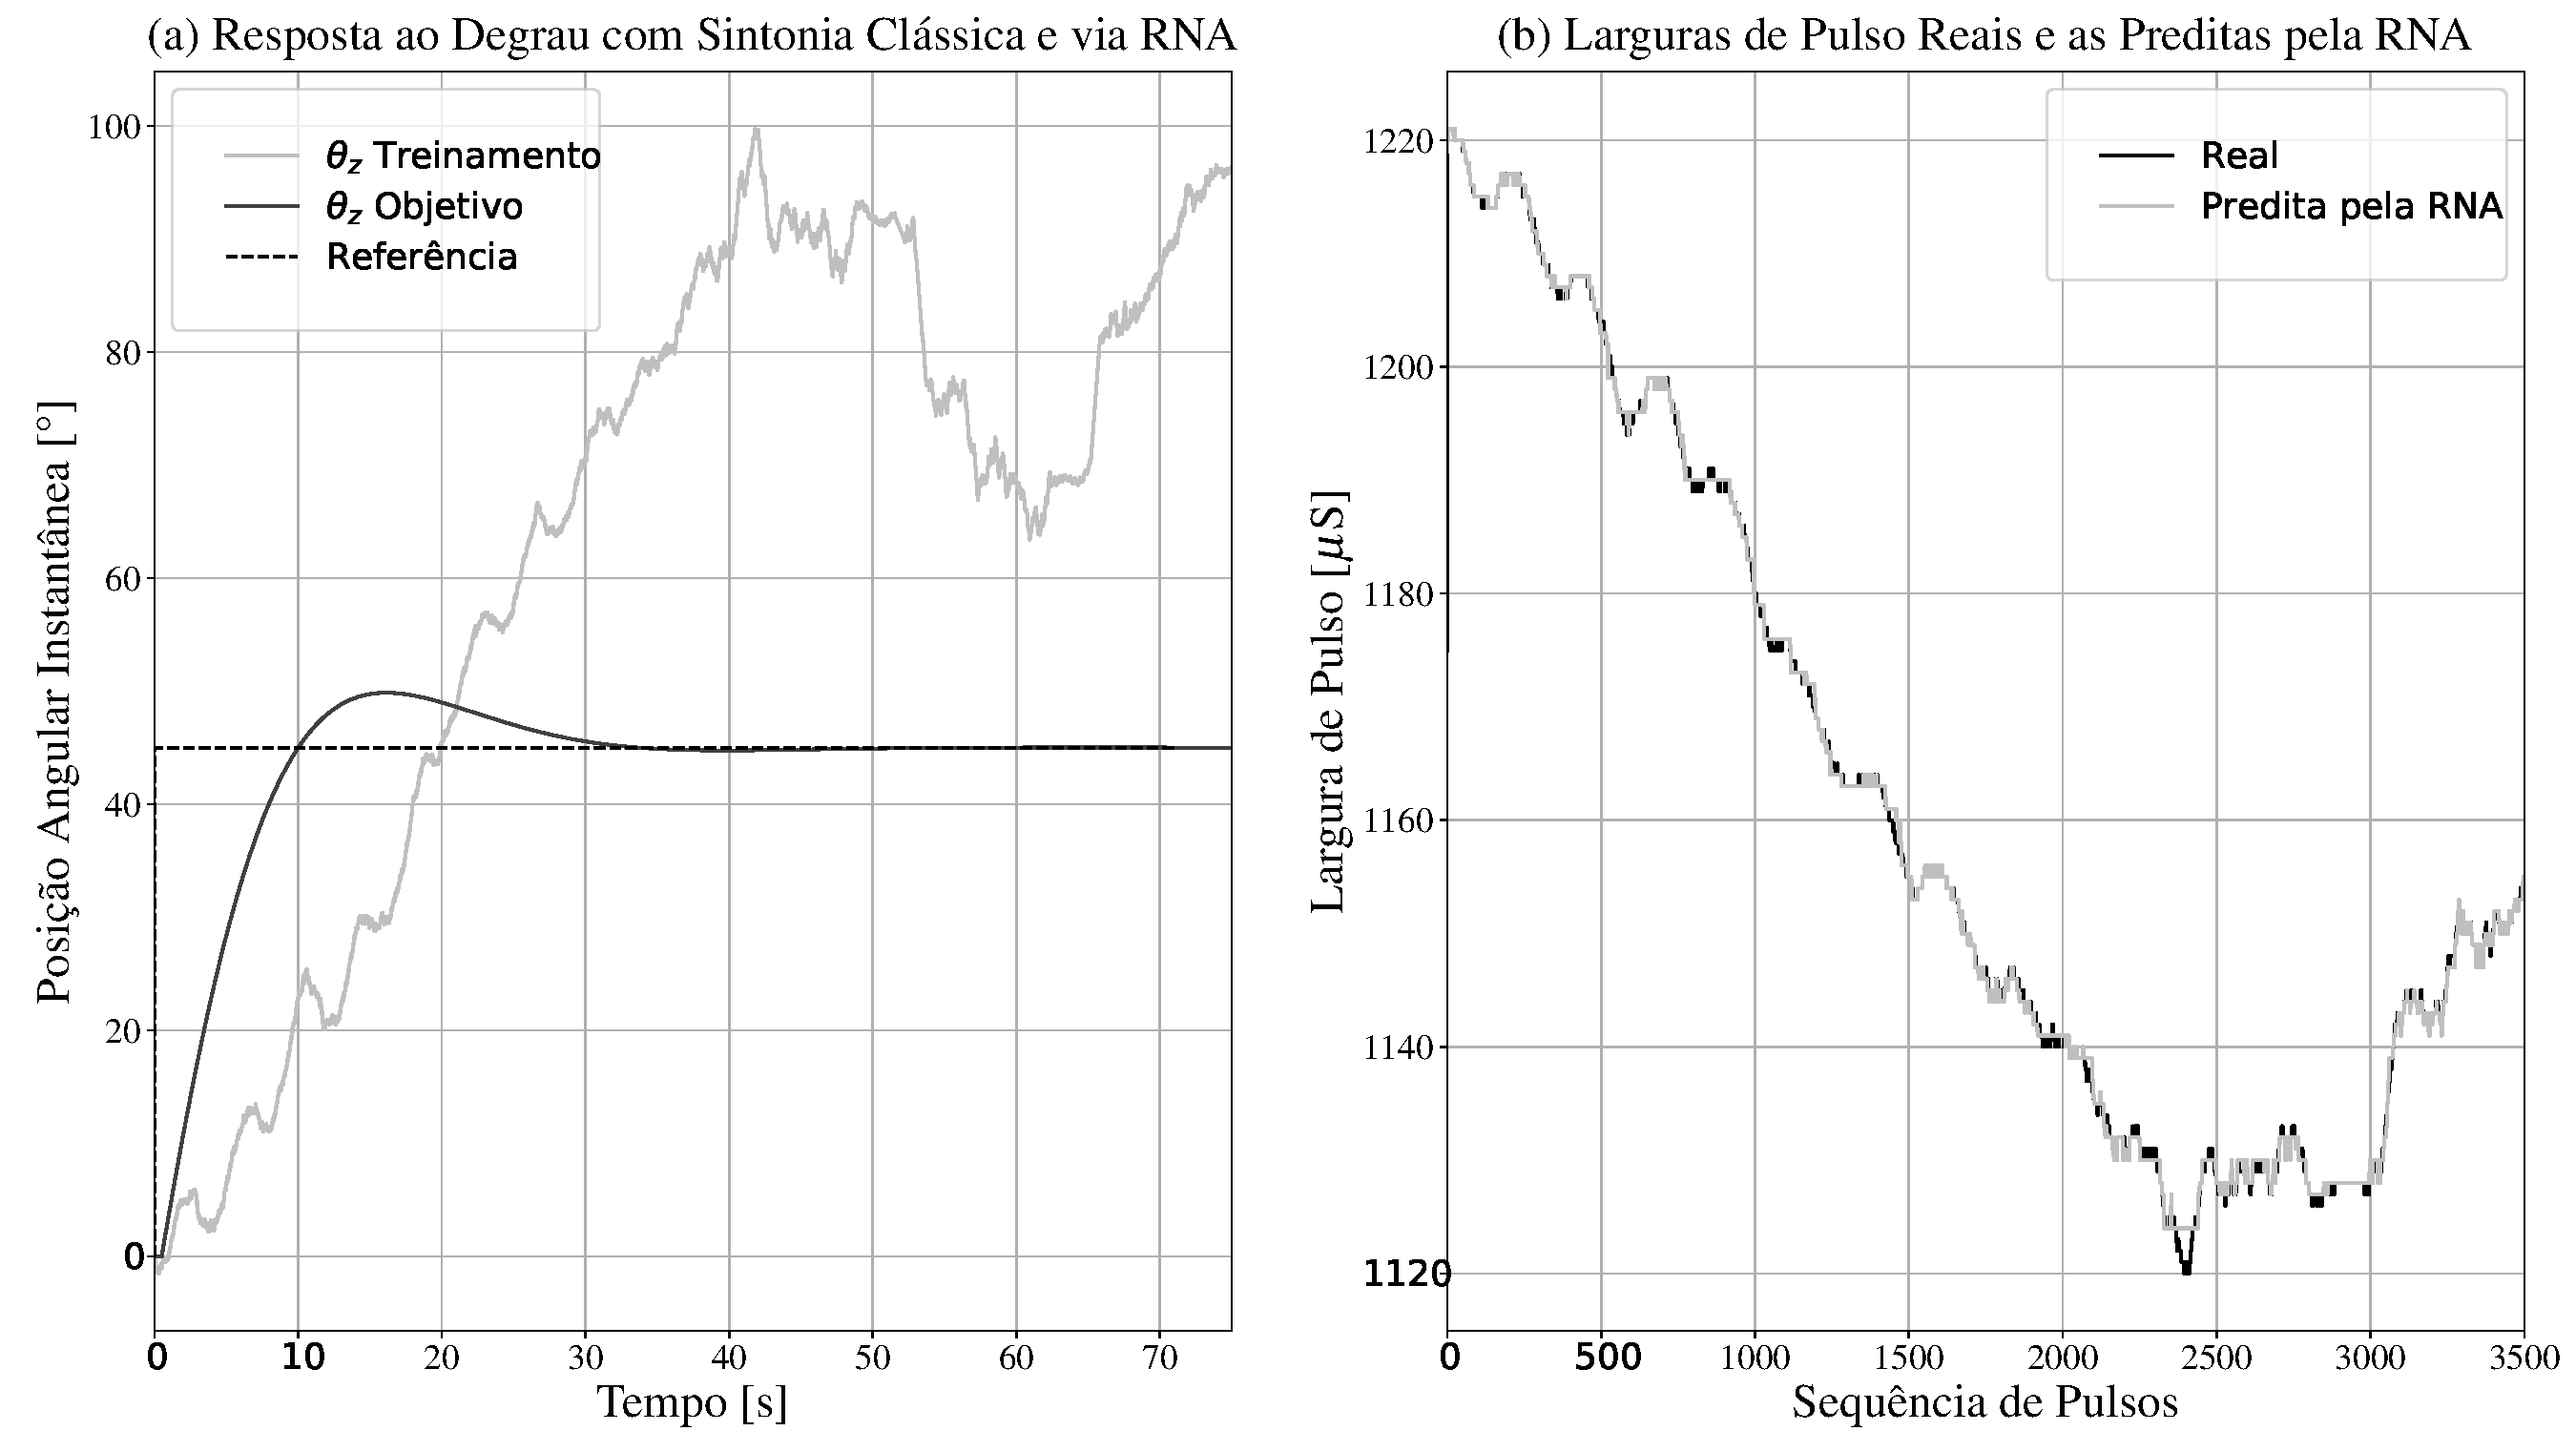
\includegraphics[scale=.22]{../resultados/img/neural_output}
        \caption{Saída da RNA treinada e o sinal real. \newline
        		 Fonte: Elaborado pelo autor.}
		\label{FIG_ADAPTATIVO}
        \end{center}
	\end{figure}
\end{frame}

%%%%%%%%%%%%%%%%%%%%%%%%%%%%%%%%%%%

\begin{frame}{Análise dos Resultados - Treinamento da RNA}
	\begin{itemize}
		\item Após o treinamento, podemos calcular o RMSE (Root Mean Square Error - Erro quadrático médio) entre os valores preditos e os amostrados, isso se dá da seguinte forma:
	\end{itemize}
\begin{equation}
RMSE = \sqrt{\frac{\sum_{t=1}^{T}(\hat{y}_t-y_t)^2}{T}}
\end{equation}
	\begin{itemize}
		\item Onde T o número de amostras, $\hat{y}_t$ são os valores preditos pela RNA e $y_t$ são os valores reais. Assim obtemos o seguinte RMSE para a rede treinada:
	\end{itemize}
\begin{equation}
RMSE \approx 1.0112
\end{equation}
\end{frame}

%%%%%%%%%%%%%%%%%%%%%%%%%%%%%%%%%%%

\begin{frame}{Análise dos Resultados - Método do Relé}
     \begin{figure}[HT]
		\begin{center}
		\captionsetup{justification=centering}
        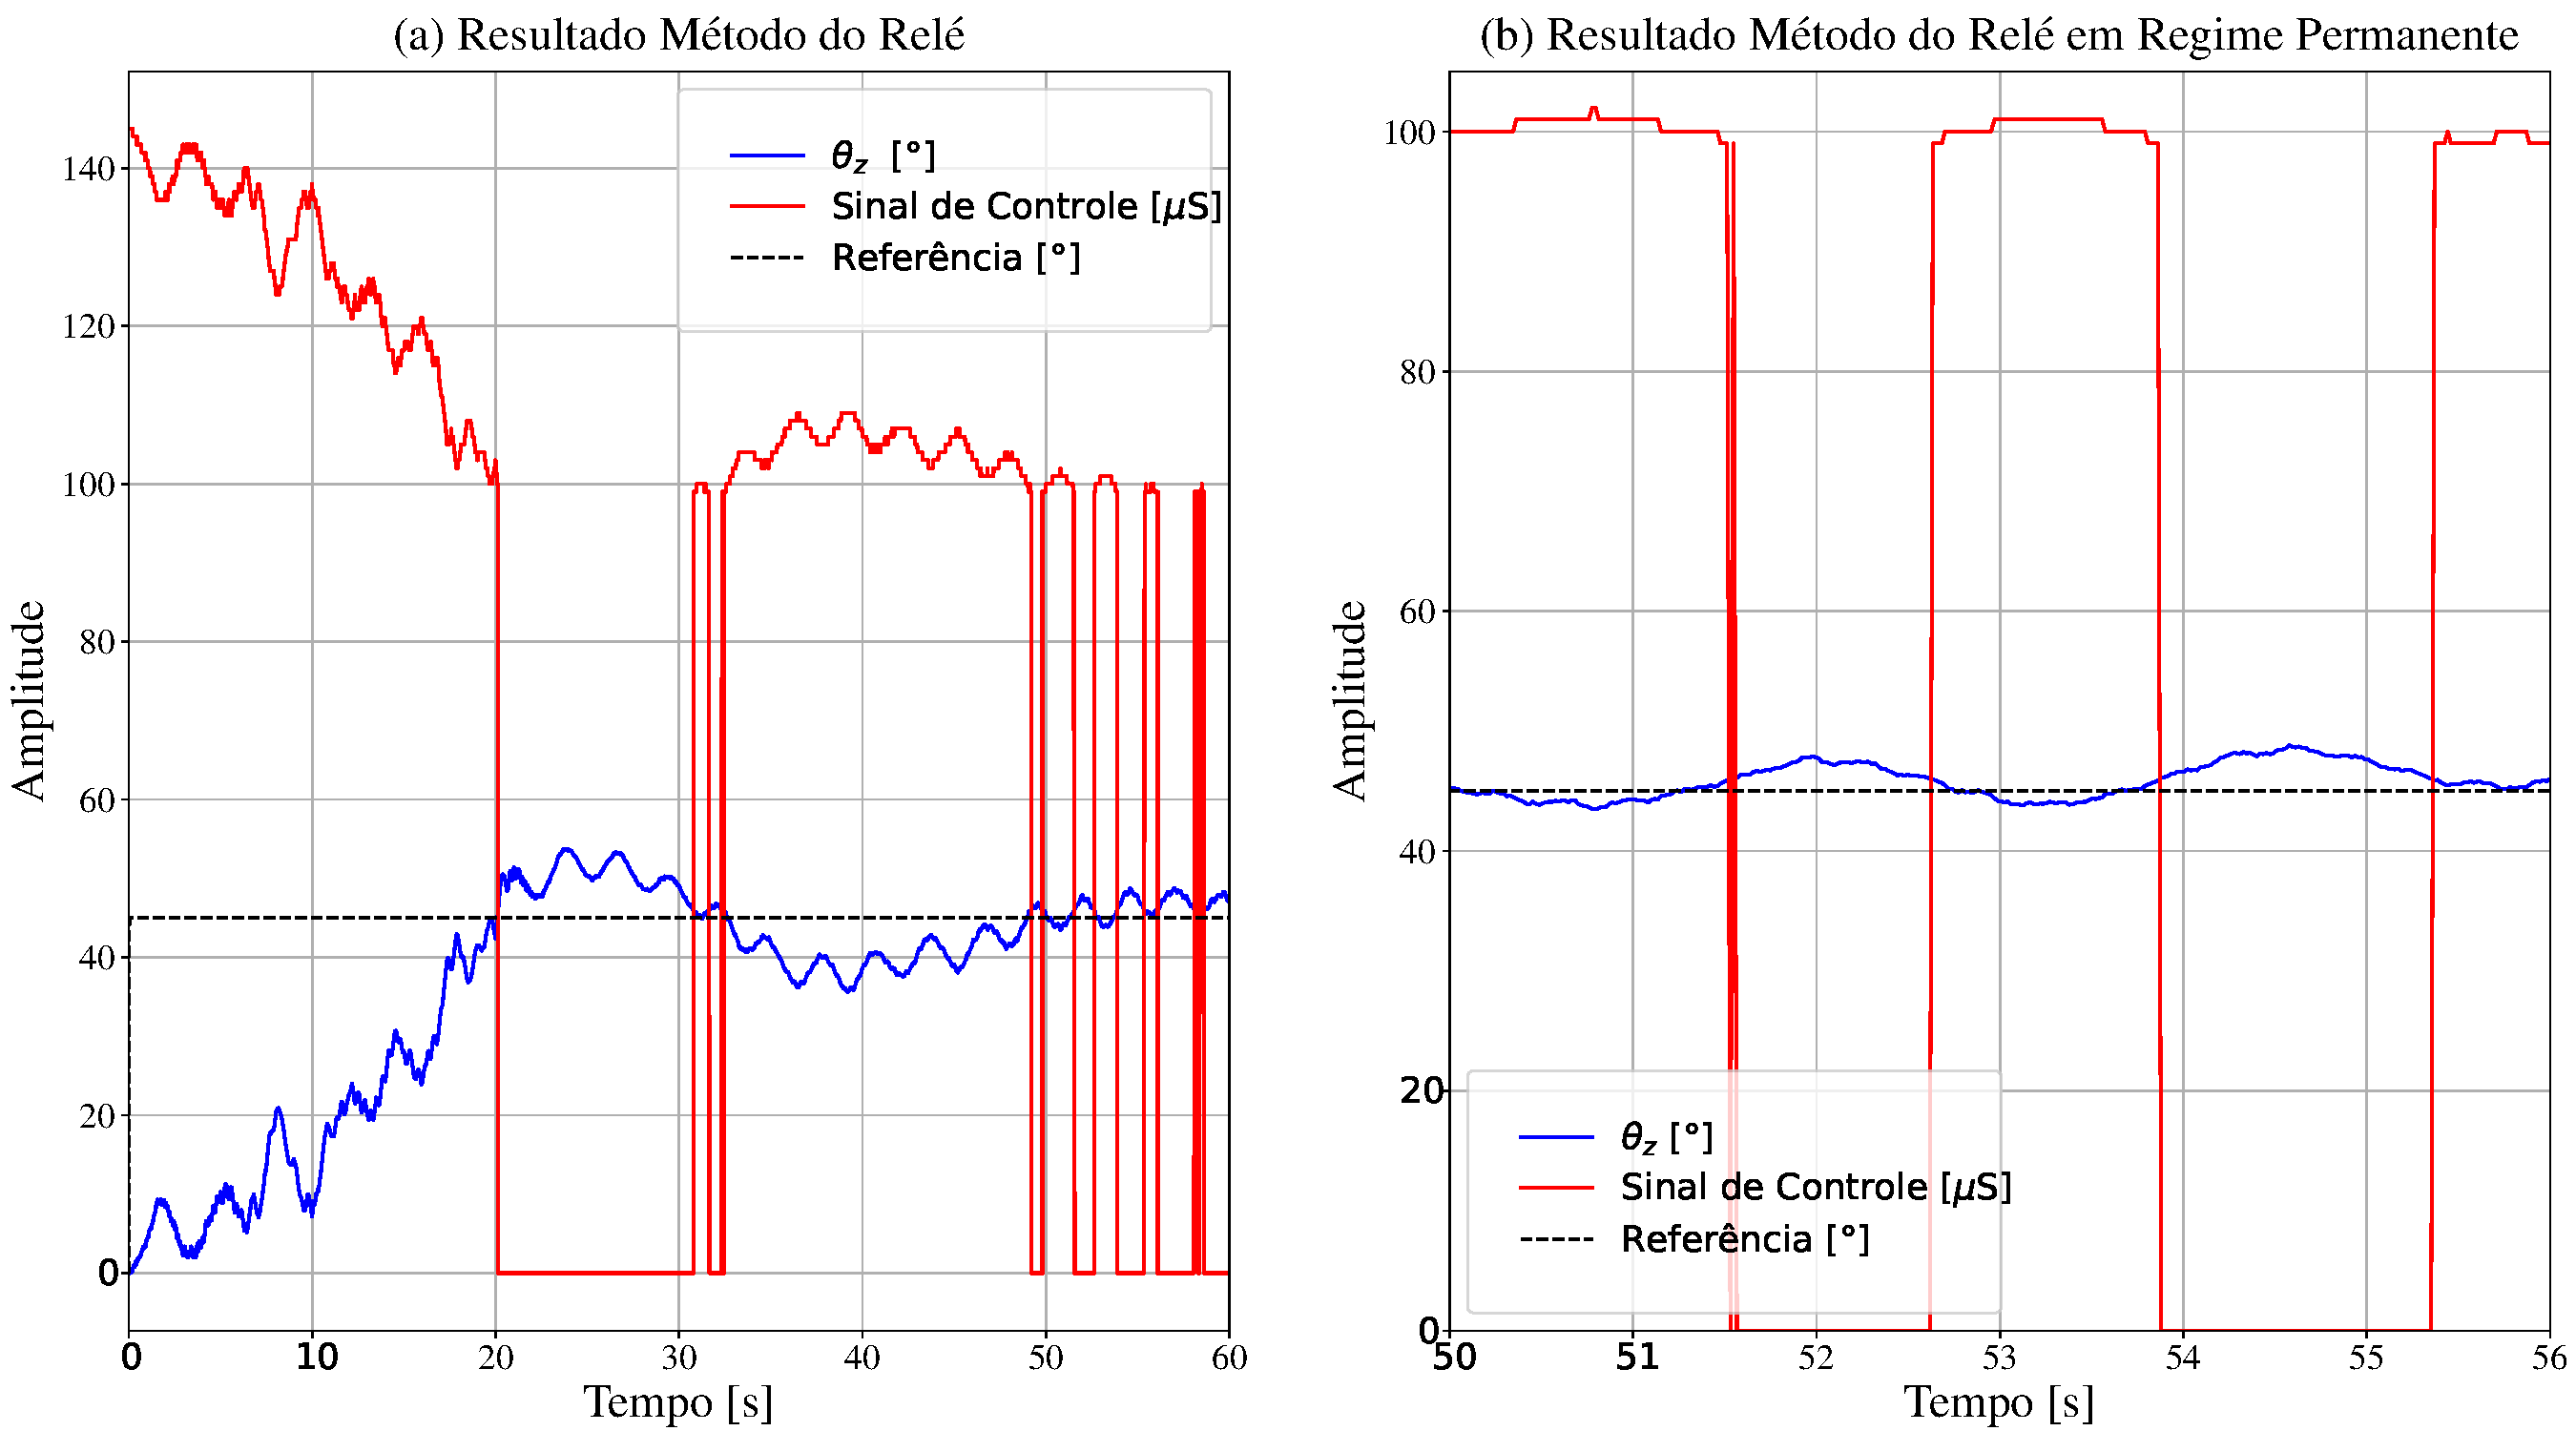
\includegraphics[scale=.22]{../resultados/img/relay}
        \caption{Resultados do método do relé. \newline
        		 Fonte: Elaborado pelo autor.}
		\label{FIG_ADAPTATIVO}
        \end{center}
	\end{figure}
\end{frame}

%%%%%%%%%%%%%%%%%%%%%%%%%%%%%%%%%%%

\begin{frame}{Análise dos Resultados - Respostas ao degrau}
     \begin{figure}[HT]
		\begin{center}
		\captionsetup{justification=centering}
        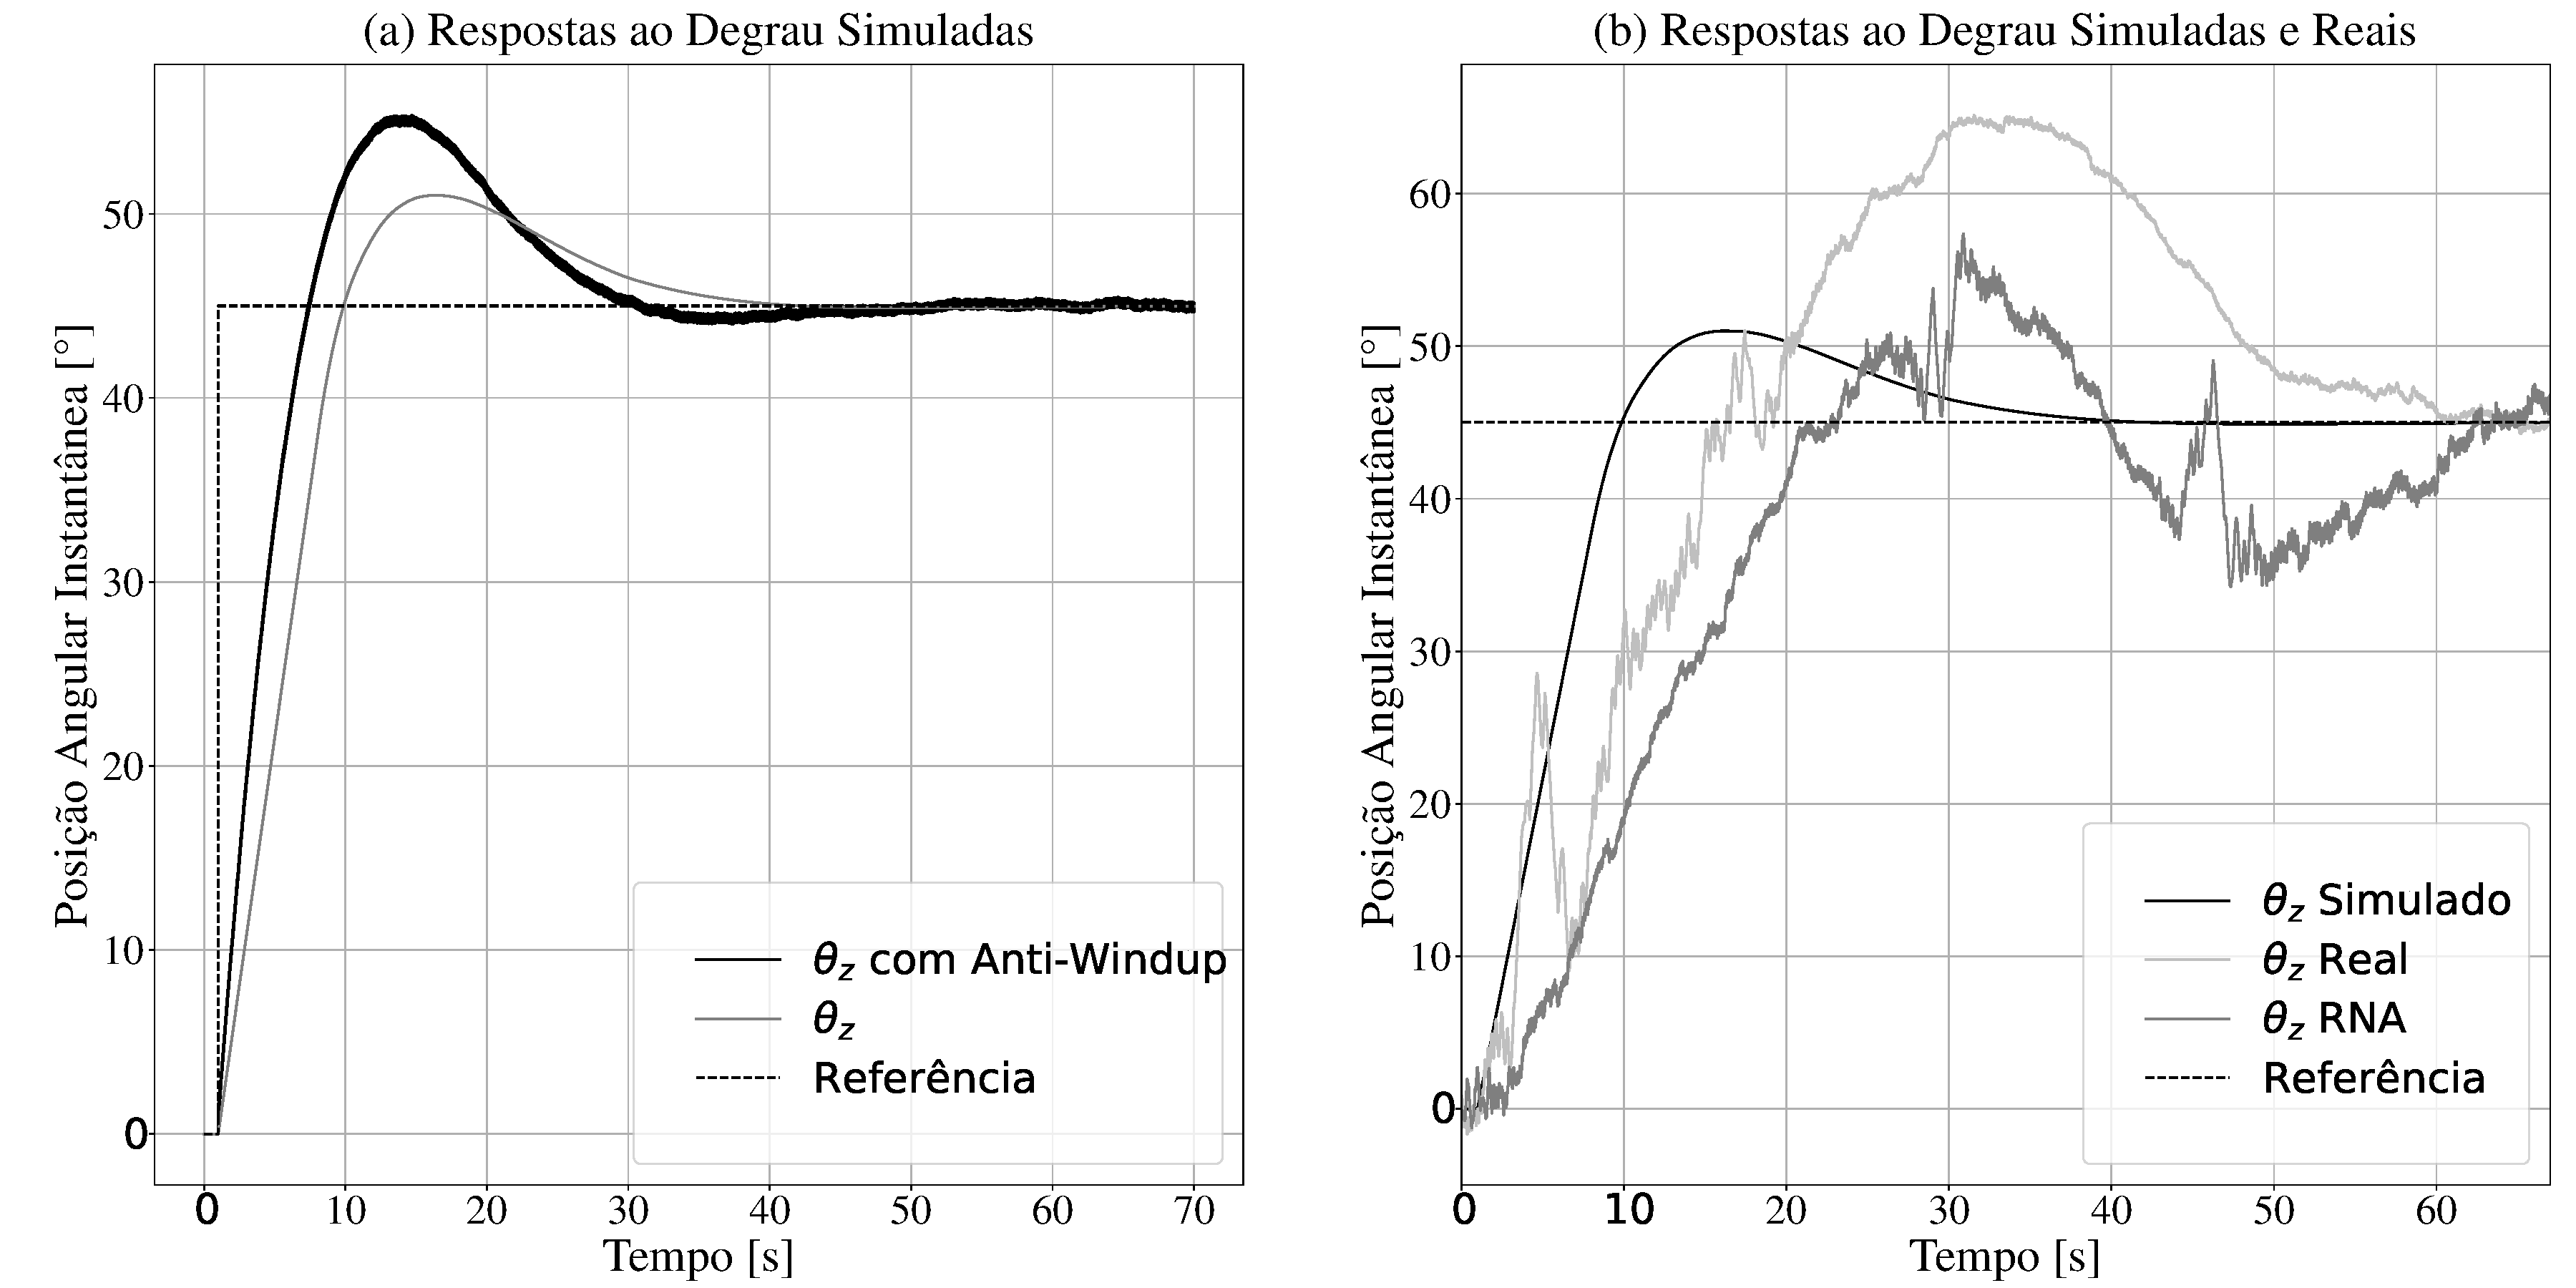
\includegraphics[scale=.18]{../resultados/img/pid_result}
        \caption{Respostas ao degrau com sintonia via método do relé. \newline
        		 Fonte: Elaborado pelo autor.}
		\label{FIG_ADAPTATIVO}
        \end{center}
	\end{figure}
\end{frame}

%%%%%%%%%%%%%%%%%%%%%%%%%%%%%%%%%%%

\begin{frame}{Análise dos Resultados - Respostas ao degrau}
     \begin{figure}[HT]
		\begin{center}
		\captionsetup{justification=centering}
        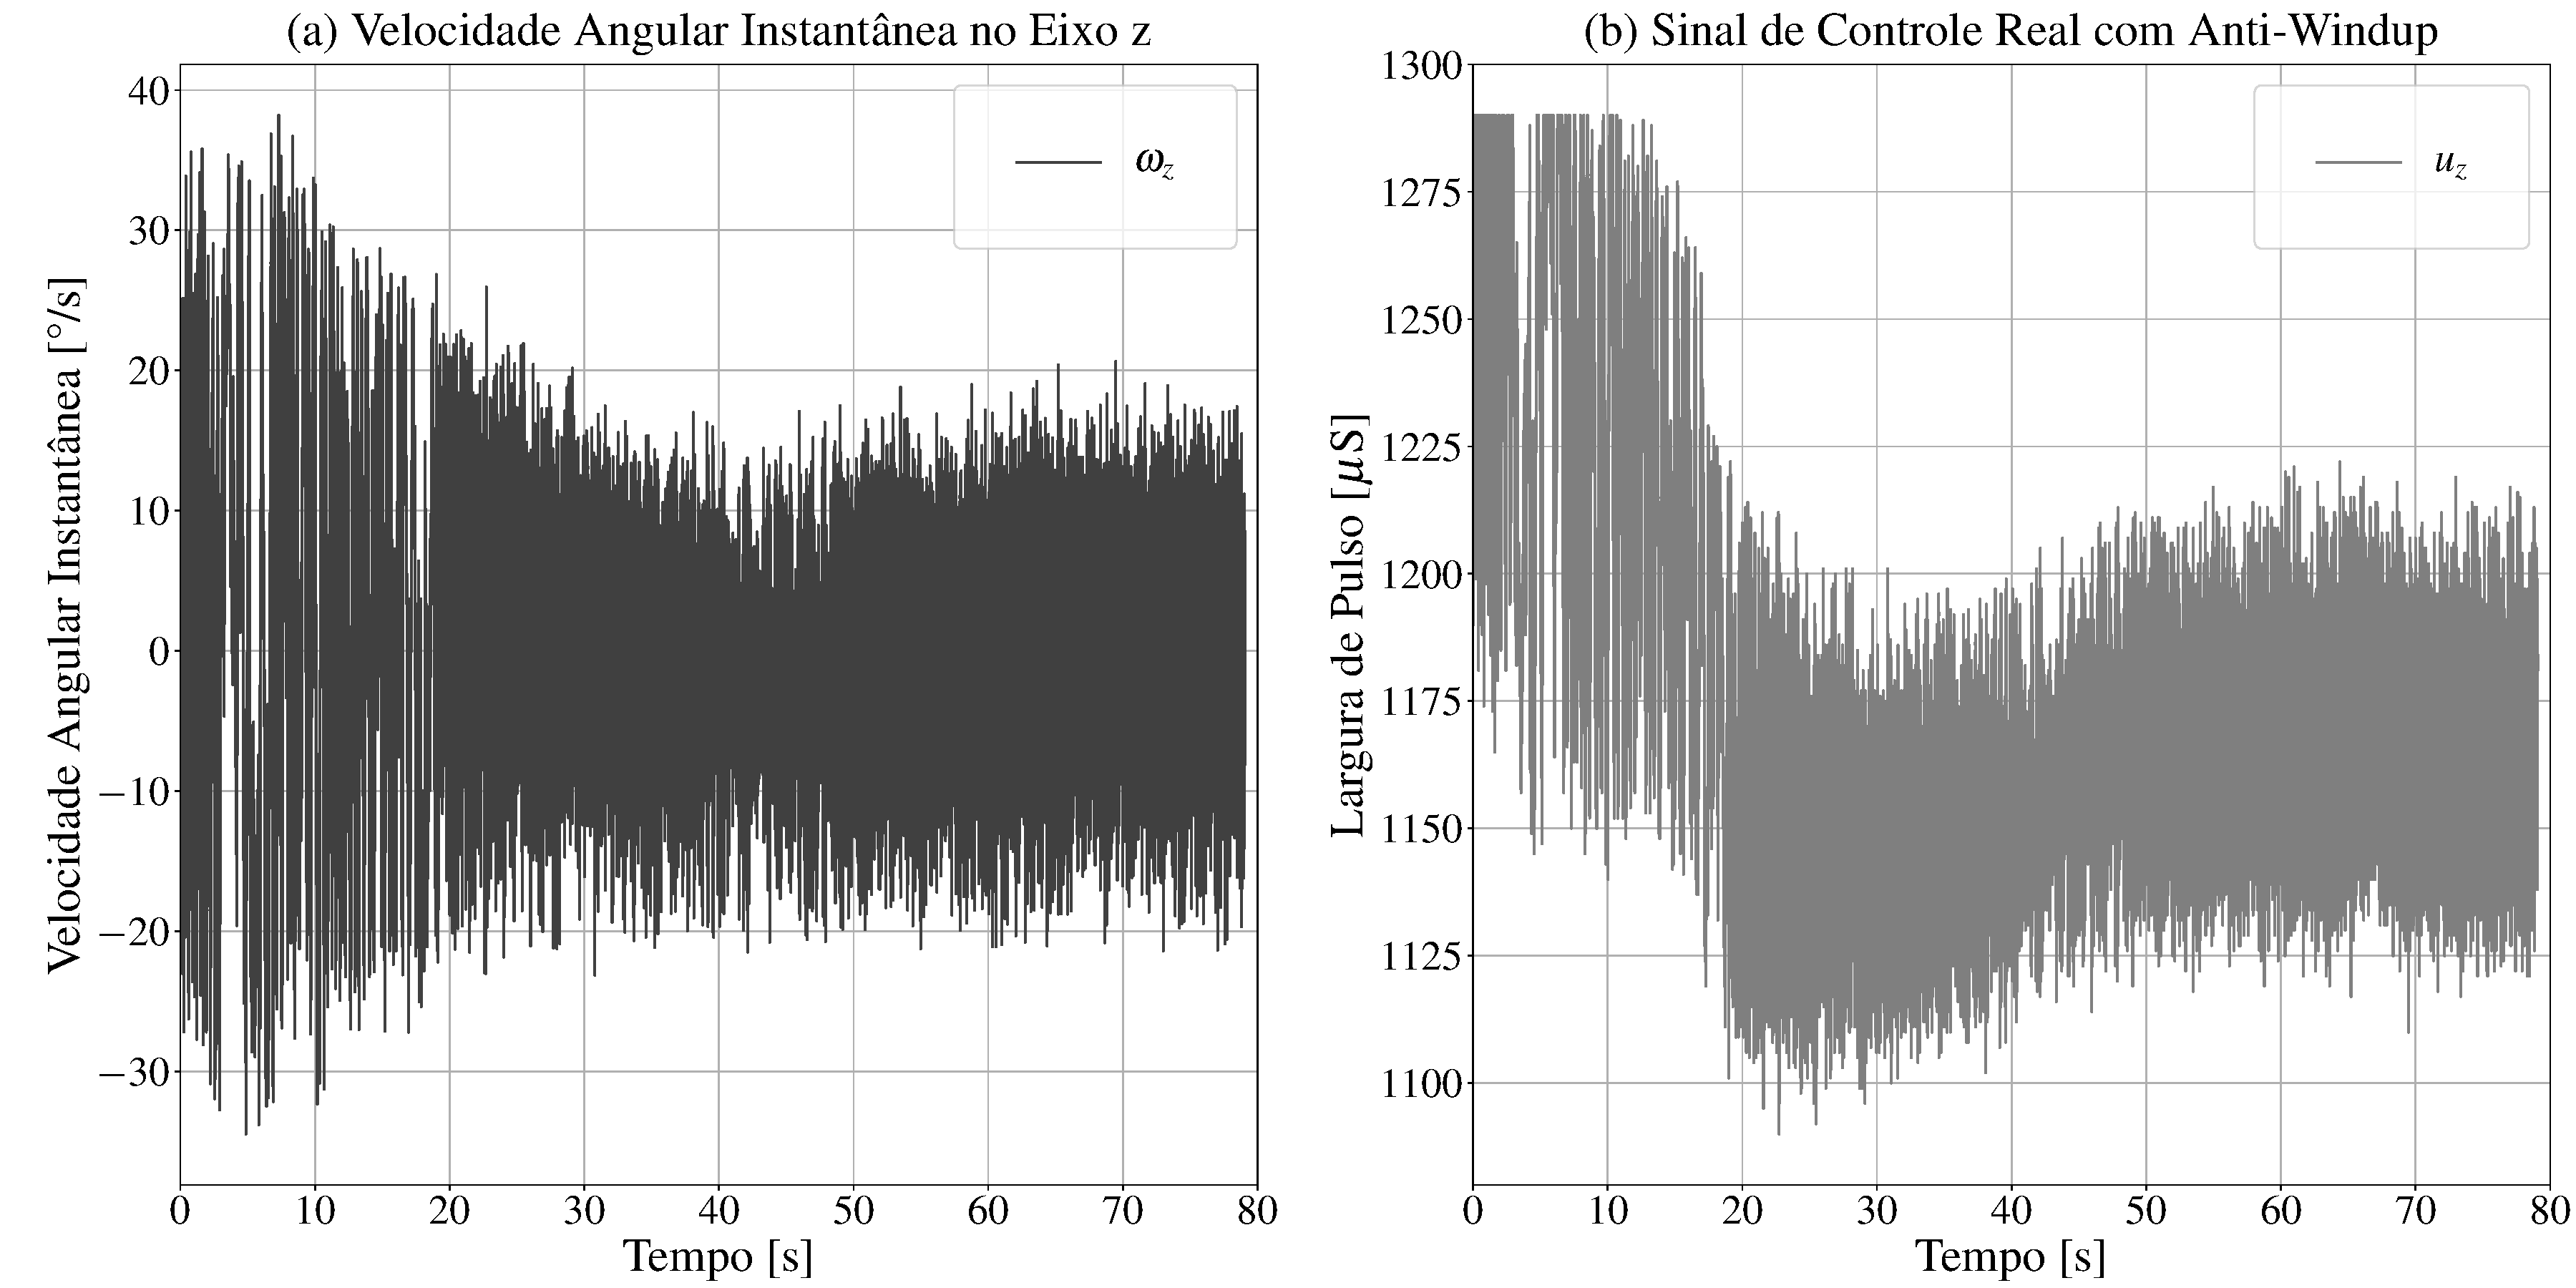
\includegraphics[scale=.18]{../resultados/img/pid_result_controller}
        \caption{Velocidade angular instantânea e sinal de controle. \newline
        		 Fonte: Elaborado pelo autor.}
		\label{FIG_ADAPTATIVO}
        \end{center}
	\end{figure}
\end{frame}

%%%%%%%%%%%%%%%%%%%%%%%%%%%%%%%%%%%

\section{Conclusão}
	\begin{frame}{Conclusão}
    \begin{itemize}
        	\justifying
			\item Perceptível influência da vibração dos motores na resposta do movimento de rotação do sumulador.
			\item Necessidade de melhorias no sistema inercial.
			\item Possibilidade de se empregar técnicas modernas em controle, onde uma RNA aprendeu o comportamento de dinâmica de um simulador de satélites.
		\end{itemize}
\end{frame}

%%%%%%%%%%%%%%%%%%%%%%%%%%%%%%%%%%%

\begin{frame}{Conclusão - Trabalhos futuros}
    \begin{itemize}
        \justifying
		\item Substituição do inercial simples por um absoluto com processamento integrado. 
		\item Criação de um interface gráfica para o usuário.
		\item Essa interface ser didática, auxiliando o ensino da teoria de controle.  
		\item Disponibilizar todos os códigos fonte no GitHub e Bitbucket.
		\end{itemize}
\end{frame}

%%%%%%%%%%%%%%%%%%%%%%%%%%%%%%%%%%%

\section{Referências Bibliográficas}
\begin{frame}{Referências Bibliográficas}
	\bibliography{../referencial/references}
\end{frame}
        
%%%%%%%%%%%%%%%%%%%%%%%%%%%%%%%%%%%

\begin{frame}{Agradecimentos}
	\begin{itemize}
        \justifying
        	\item Ao meu orientador Rodrigo Marques de Figueiredo. 
        	\item Aos professores Walter Andrey Fontana e Dilson Jose Aguiar de Souza.
			\item Aos laboratoristas dos laboratórios da Eng. Mecânica.
			\item Aos laboratoristas dos laboratórios da Eng. Elétrica.
			\item Aos demais amigos e familiares que, de alguma forma, ajudaram na elaboração desse trabalho.  
		\end{itemize}
	\end{frame}

%%%%%%%%%%%%%%%%%%%%%%%%%%%%%%%%%%%

\begin{frame}{Agradecimentos}
		\begin{center}
			{\Huge Obrigado pela Atenção!}
		\end{center}
\end{frame}

\end{document}